\begin{figure}[h!]
	\centering
	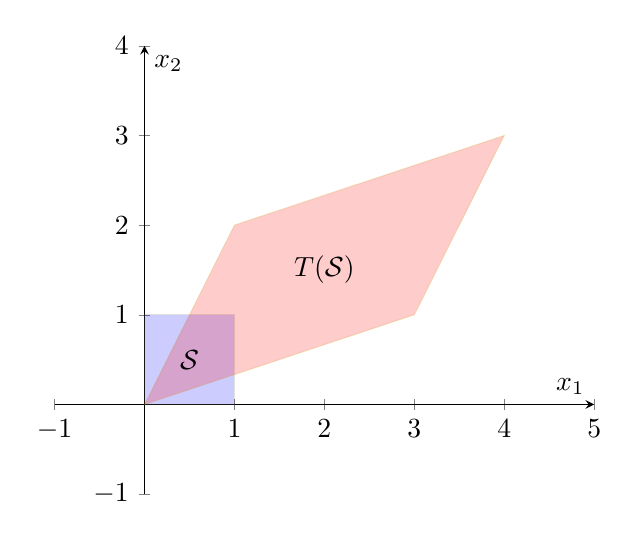
\begin{tikzpicture}
		\begin{axis}[xlabel=$x_1$, ylabel=$x_2$, axis x line=middle, axis y line=middle, xmin=-1, ymin=-1, xmax=5, ymax=4]

		\addplot[surf,mesh/rows=2, patch type=rectangle, blue, opacity=0.2] coordinates {(0,0) (1,0) (0,1) (1,1)};
		
		\addplot[surf,mesh/rows=2, patch type=rectangle, red, opacity=0.2] coordinates {(0,0) (1,2) (3,1) (4,3)};
		
		\node[draw=none, fill=none] at (axis cs:0.5,0.5) {$\mathcal{S}$} ;
		\node[draw=none, fill=none] at (axis cs:2,1.5) {$T(\mathcal{S})$} ;
		\end{axis}
	\end{tikzpicture}
	\caption{Grafische weergave van het voorbeeld}
	\label{fig:linafb}
\end{figure}